\section{Network Inference}

\pgfdeclareimage[height=0.8\textheight]{sparsity1}{figures/sparsity_1}
\pgfdeclareimage[height=0.8\textheight]{sparsity2}{figures/sparsity_2}
\pgfdeclareimage[height=0.375\textheight]{sparsity4}{figures/sparsity_4}

\begin{frame}
  \frametitle{References}

    \begin{thebibliography}{99}
      \setbeamertemplate{bibliography item}[book]

    \bibitem[JC]{JC} Habilitation, J. Chiquet, Chapter 2 \href{https://tel.archives-ouvertes.fr/tel-01288976/}{https://tel.archives-ouvertes.fr/tel-01288976/}
    \bibitem[EI]{EI} The Element of Statistical Learning \textcolor{black}{Hastie, Tibshirani, Friedman}, chapter 17.
    \end{thebibliography}

\end{frame}

\begin{frame}
  \frametitle{Some families of methods for network reconstruction}

  \begin{block}{Test-based methods}
    \vspace{-.15cm}
    \begin{itemize}
    \item Tests the nullity of each entries 
    \item Combinatorial problem when $p>30$ \dots
    \end{itemize}    
  \end{block}
  
  \vfill

  \begin{block}{Bayesian methods}
    \vspace{-.15cm}
    \begin{itemize}
    \item Compute the posterior probability of each edge
    \item Usually more computationally demanding
    \item For special graphs, computation gets easier
    \end{itemize}
  \end{block}

  \begin{block}{\alert{Sparsity-inducing regularization methods}}
    \vspace{-.15cm}
    \begin{itemize}
    \item induce sparsity with the $\ell_1$-norm penalization
    \item Use results from convex optimization
    \item Versatile and computationally efficient
    \end{itemize}
  \end{block}

\end{frame}

\subsection{Inducing sparsity for edge selection}

\begin{frame}
  \frametitle{Inference: maximum likelihood estimator}
  \framesubtitle{The natural approach for parametric statistics}

  Let   $X\sim f_{X}(x;\boldsymbol\Omega)$,  where   $\boldsymbol\Omega$  are  the
  model parameters.

  \vfill

  \begin{block}{Maximum likelihood estimator}
    \begin{equation*}
      \hat{\boldsymbol\Omega}      =      \argmax_{\boldsymbol\Omega}
      \ell(\boldsymbol\Omega; \mathbf{X})
    \end{equation*}
    where  $\ell$ is  the log  likelihood, a  function  of the
    parameters:
    \begin{equation*}
      \ell(\boldsymbol\Omega;      \mathbf{X})      =     \log
      \prod_{i=1}^n f_{X}(\mathbf{x}_i;\boldsymbol\Omega),
    \end{equation*}
    where $\mathbf{x}_i$ is the $i$th row of $\mathbf{X}$.
  \end{block}

  \vfill
  
  \begin{itemize}
    \item This a convex optimization problem,
    \item We just need to detect non zero coefficients in $\boldsymbol\Omega$
  \end{itemize}

\end{frame}

\begin{frame}
  \frametitle{The multivariate Gaussian log-likelihood }

  Let  $\mathbf{S}  =  n^{-1}\mathbf{X}^\intercal \mathbf{X}$  be  the
  empirical variance-covariance  matrix: $\mathbf{S}$ is  a sufficient
  statistic of $ \boldsymbol\Omega$.

  \vfill

  \begin{block}{The log-likelihood}
    \begin{equation*}
      \ell(\boldsymbol\Omega; \mathbf{S}) =
      \frac{n}{2}     \log    \det     (\boldsymbol\Omega)  - \frac{n}{2}
      \mathrm{Trace}(\mathbf{S} \boldsymbol\Omega) + \frac{n}{2}\log(2\pi).
    \end{equation*}
  \end{block}

  \vfill

  \begin{itemize}
  \item[$\rightsquigarrow$]    The     MLE    $=\mathbf{S}^{-1}$    of
    $\boldsymbol\Omega$ is not defined for $n< p$ and never sparse.
  \item[$\rightsquigarrow$] The need for regularization is huge.
  \end{itemize}
\end{frame}

\begin{frame}
  \frametitle{A Geometric View of Shrinkage}
  \framesubtitle{Constrained Optimization}

  \begin{overlayarea}{\textwidth}{\textheight}
    \begin{columns}
      \begin{column}{0.475\textwidth}
        \begin{tikzpicture}
          \only<1>{%
            \node (Surf) at (0,0) {\pgfuseimage{sparsity1}}
            node     at    (Surf.west)    [rotate=90,yshift=5mm]
            {$L(\Omega_1,\Omega_2;\mathbf{X})$}
            node at (Surf.south west) [xshift=5mm,yshift=5mm]{$\Omega_2$}
            node at (Surf.south east) [xshift=-7.5mm,yshift=2.5mm]{$\Omega_1$};
          }
          \only<2>{%
            \node (Surf2) at (0,0) {\pgfuseimage{sparsity2}}
            node    at    (Surf2.west)    [rotate=90,yshift=5mm]
            {$L(\Omega_1,\Omega_2;\mathbf{X})$}
            node at (Surf2.south west) [xshift=5mm,yshift=5mm]{$\Omega_2$}
            node at (Surf2.south east) [xshift=-7.5mm,yshift=2.5mm]{$\Omega_1$};
          }
          \only<3->{%
            \node (titi) at (0,0) {\phantom{titi}};
            \node (Surf3) at (0,-4.5) {\pgfuseimage{sparsity4}}
            node at (Surf3.west) [rotate=90,yshift=2.5mm] {$\Omega_2$}
            node at (Surf3.south) [yshift=-2.5mm] {$\Omega_1$};
          }
        \end{tikzpicture}
      \end{column}
      \begin{column}{0.55\textwidth}
        \only<1>{%
          We basically want to solve a problem of the form
          \begin{equation*}
            \maximize_{\Omega_1,\Omega_2} \ell(\Omega_1,\Omega_2;\mathbf{X})
          \end{equation*}
          where $\ell$ is typically a concave likelihood function.
        }
        \only<2->{%
          \begin{equation*}
            \left\{\begin{array}{ll}
                \displaystyle    \maximize_{\Omega_1,\Omega_2}   &
                \ell(\Omega_1,\Omega_2;\mathbf{X})\\
                \mathrm{s.t.} & \Omega(\Omega_1,\Omega_2) \leq c
              \end{array}\right.,
          \end{equation*}
          where  $\Omega$  defines  a  domain  that  \textit{constrains}
          $\boldsymbol\beta$.

          \begin{center}
            How shall we define $\Omega$ ?
          \end{center}
        }
      \end{column}
    \end{columns}
  \end{overlayarea}
\end{frame}


\pgfdeclareimage[height=0.375\textheight]{sparsity6}{figures/sparsity_6}
\pgfdeclareimage[height=0.375\textheight]{sparsity8bis}{figures/sparsity_8bis}
\pgfdeclareimage[height=0.375\textheight]{sparsity9}{figures/sparsity_9}
\pgfdeclareimage[height=0.375\textheight]{sparsity10}{figures/sparsity_10}
\pgfdeclareimage[height=0.375\textheight]{sparsity11}{figures/sparsity_11}
\pgfdeclareimage[height=0.375\textheight]{sparsity12}{figures/sparsity_12}


\begin{frame}
  \frametitle{A Geometric View of Sparsity}
  \framesubtitle{Dual and Polar Cones}

  {\centerline{Generalizes normals}}

  \bigskip

  \begin{overlayarea}{\textwidth}{\textheight}


    \begin{tikzpicture}
      \only<1>{%
      \node (Surf2) at (0,0) {\pgfuseimage{sparsity6}}
              node at (Surf2.west) [rotate=90,yshift=2.5mm] {$\beta_2$}
              node at (Surf2.south) [yshift=-1mm] {$\beta_1$};
      }
      \only<1-2>{%
      \node (Surf3) at (4,0) {\pgfuseimage{sparsity8bis}}
              node at (Surf3.west) [rotate=90,yshift=2.5mm] {$\beta_2$}
              node at (Surf3.south) [yshift=-1mm] {$\beta_1$};
      }
      \only<1-3>{%
        \node (Surf4) at (8,0) {\pgfuseimage{sparsity9}}
                node at (Surf4.west) [rotate=90,yshift=2.5mm] {$\beta_2$}
                node at (Surf4.south) [yshift=-1mm] {$\beta_1$};
      }
      \only<4>{%
        \node (Surf5) at (8,0) {\pgfuseimage{sparsity10}}
                node at (Surf5.west) [rotate=90,yshift=2.5mm] {$\beta_2$}
                node at (Surf5.south) [yshift=-1mm] {$\beta_1$};
      }
      \only<3->{%
        \node (Surf6) at (4,0) {\pgfuseimage{sparsity11}}
                node at (Surf6.west) [rotate=90,yshift=2.5mm] {$\beta_2$}
                node at (Surf6.south) [yshift=-1mm] {$\beta_1$};
      }
      \only<2->{%
        \node (Surf7) at (0,0) {\pgfuseimage{sparsity12}}
                node at (Surf7.west) [rotate=90,yshift=2.5mm] {$\beta_2$}
                node at (Surf7.south) [yshift=-1mm] {$\beta_1$};
      }
    \end{tikzpicture}

    \medskip

    Let $C$ be a convex set,
    \begin{itemize}
    \item  $C^\star(x_0) =  \set{y|y^T(x-x_0) \geq  0,x\in C}$  is the
      dual cone in $x_0$,
    \item $N_C(x_0) = \set{y|y^T(x-x_0) \leq 0,x\in C}$ is the polar (or normal) cone, 
    \end{itemize}

    \medskip

    \only<4>{%
      {\centerline{Shape of cones $\Rightarrow$ sparsity pattern}}
    }

  \end{overlayarea}
\end{frame}

\begin{frame}
  \frametitle{The Lasso}
  \framesubtitle{Least Absolute Shrinkage and Selection Operator}

  \begin{block}{Idea}
    Suggest  an admissible  set that  induces  \alert{sparsity} (force
    several entries to exactly zero in $\hat{\bbeta}$).
  \end{block}

  \vfill

  \begin{overlayarea}{\textwidth}{.4\textheight}
    \begin{columns}
      \begin{column}[c]{.6\textwidth}
        \begin{block}{Lasso as a regularization problem}
          The Lasso estimate of $\bbeta$ is the solution to
          \begin{equation*}
            \hat{\btheta}^{\text{lasso}}     =    \argmin_{\btheta}
            -\ell(\btheta),  \quad   \text{s.t.  }  \sum_{j=1}^p
            \left|\Omega_j\right|
            \leq s,
          \end{equation*}
          where $s$ is a shrinkage factor.
        \end{block}
      \end{column}
      \begin{column}{.4\textwidth}
        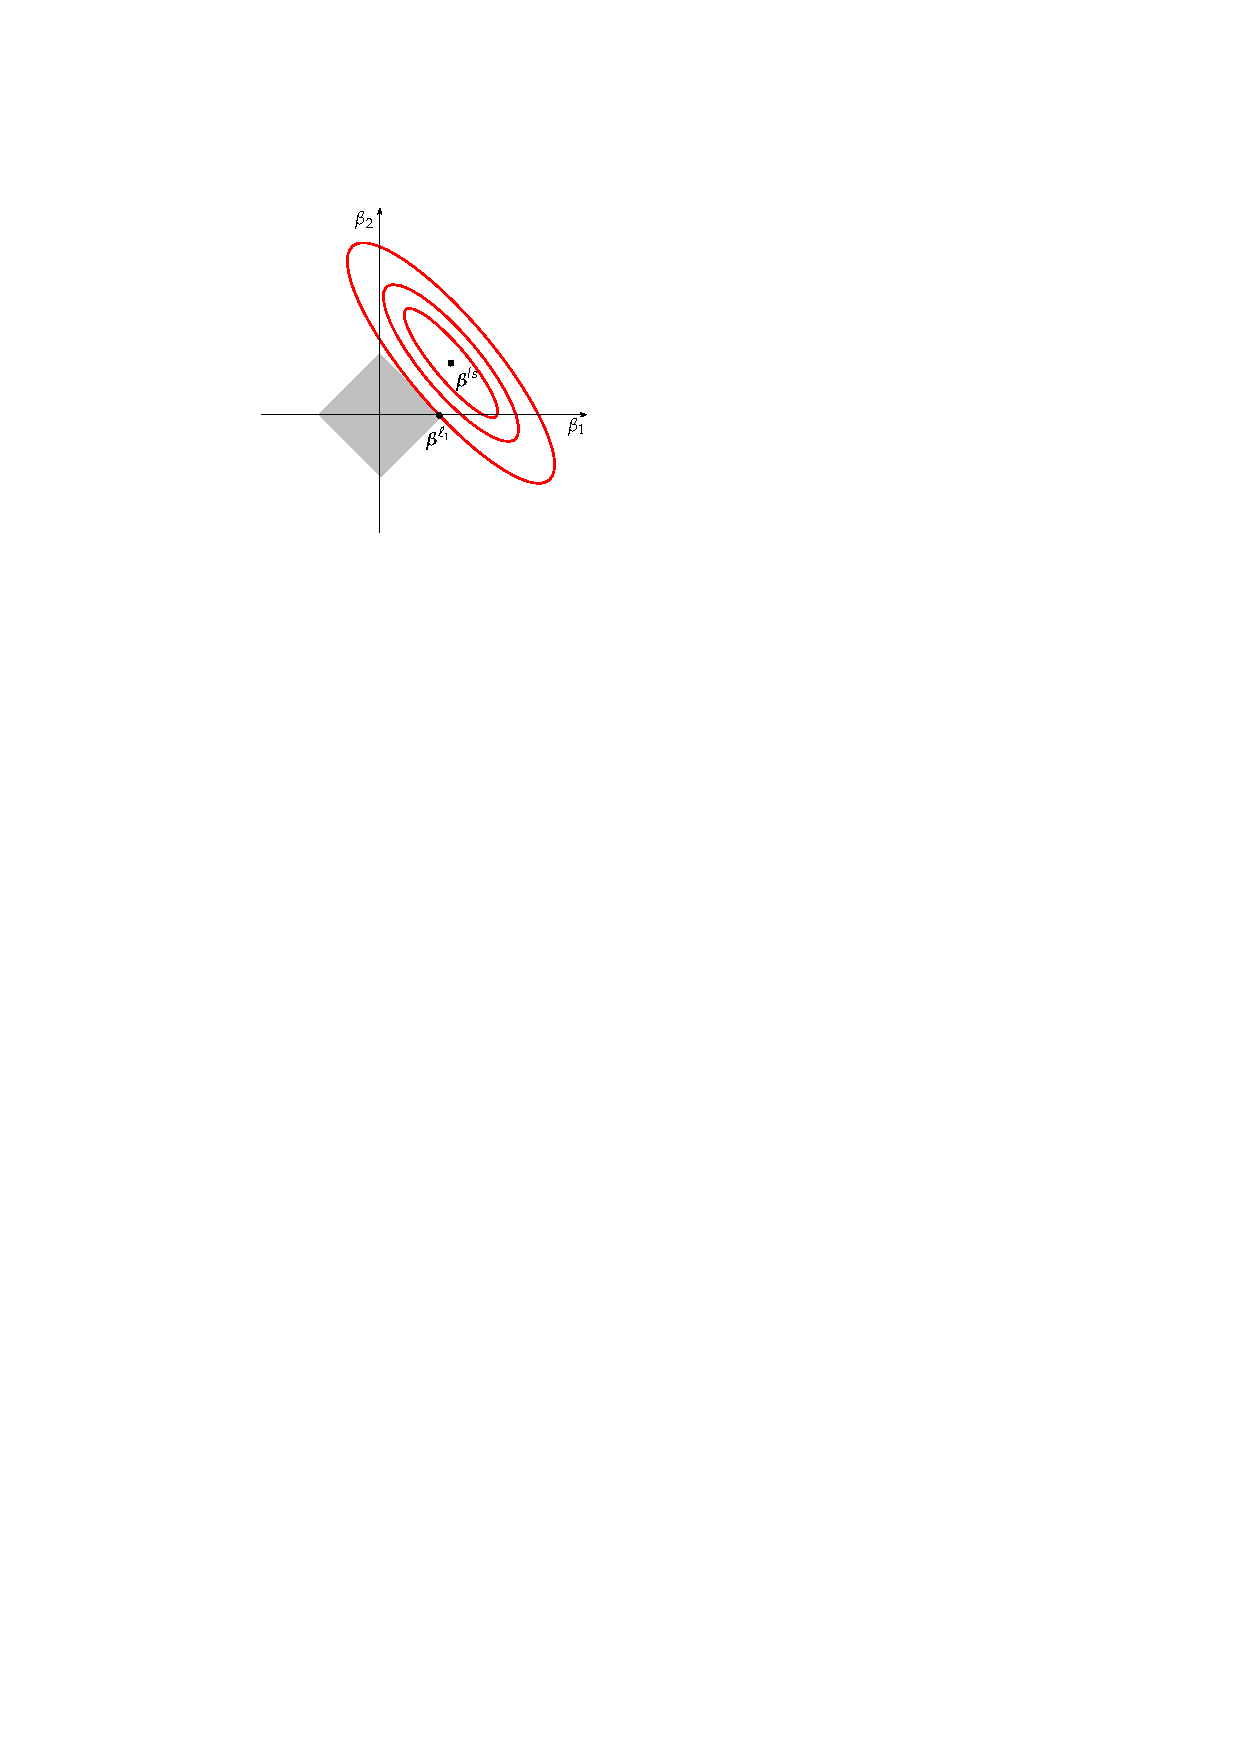
\includegraphics[width=.75\textwidth]{figures/lasso_set}
      \end{column}
    \end{columns}
  \end{overlayarea}

\end{frame}

\begin{frame}
  \frametitle{Insights: 2-dimensional example with the square loss}

  \begin{overlayarea}{\textwidth}{\textheight}

    \begin{equation*}
      \sum_{i=1}^n (y_i-x_i^1\Omega_1 - x_i^2\Omega_2)^2, \qquad
      \only<1>{\text{no constraints}}
      \only<2>{\text{s.t. } |\Omega_1| + |\Omega_2| < 0.75}
      \only<3>{\text{s.t. } |\Omega_1| + |\Omega_2| < 0.66}
      \only<4>{\text{s.t. } |\Omega_1| + |\Omega_2| < 0.4}
      \only<5>{\text{s.t. } |\Omega_1| + |\Omega_2| < 0.2}
      \only<6>{\text{s.t. } |\Omega_1| + |\Omega_2| < 0.0743}
    \end{equation*}

  \vspace{-.5cm}

    \includegraphics<1>[width=.8\textwidth]{dess11}
    \includegraphics<2>[width=.8\textwidth]{dess12}
    \includegraphics<3>[width=.8\textwidth]{dess13}
    \includegraphics<4>[width=.8\textwidth]{dess14}
    \includegraphics<5>[width=.8\textwidth]{dess15}
    \includegraphics<6>[width=.8\textwidth]{dess16}

  \end{overlayarea}

\end{frame}

\begin{frame}
  \frametitle{Application to GGM}

  \begin{block}{A penalized likelihood approach}
    \vspace{-1em}
    \begin{equation*}
      \hat{\bTheta}_\lambda=\argmax_{\bTheta \in \mathbb{S}_+}
      \ell(\bTheta;\mathbf{X})-\lambda
      \mathrm{pen}_{\ell_1}(\bTheta)
    \end{equation*}
  where
  \begin{itemize}
  \item $\mathcal{\ell}$ is the model log-likelihood,
  \item $\mathrm{pen}_{\ell_1}$ is a \alert{penalty function} tuned by
    $\lambda>0$.
    \vfill
      \begin{enumerate}
      \item \textit{regularization} (needed when $n \ll p$),
      \item \textit{selection} (sparsity induced by the $\ell_1$-norm).
      \end{enumerate}
  \end{itemize}
\end{block}

\end{frame}

\begin{frame}
  \frametitle{Gold standard penalized approaches}

  \vspace{-.25cm}
  
  \begin{overlayarea}{\textwidth}{\textheight}

    \begin{block}{Penalized   likelihood  (Banerjee   \textit{et
          al.}, Yuan and Lin, 2008)}
      \vspace{-1em}
      \begin{equation*}
        \hat{\bTheta}_\lambda=\argmax_{\bTheta \in \mathbb{S}_+}
        \ell(\bTheta;\mathbf{X})-\lambda
        \|\bTheta\|_{1}
      \end{equation*}
    \end{block}
    \vspace*{-1.5em}
    
    \begin{itemize}
    \item[\textcolor{green}{$+$}] symmetric, positive-definite
    \item[\textcolor{red}{$-$}]       solved      by       the
      ``Graphical-Lasso''                 ($\mathcal{O}(p^3)$,
      \textit{Friedman et al, 2007}).
    \item \texttt{R}-packages \textbf{glasso}, \textbf{quic}, \textbf{huge}.
    \end{itemize}
    
    \vfill
    
    \begin{block}{Neighborhood    Selection   (Meinshausen    \&
        B\"ulhman, 2006)}<2-> \vspace*{-1em}
      \only<2>{
         \begin{equation*}
          \text{For variable $j$, solve} \quad \hatbbeta_j  = \argmin_{\bbeta\in\Rset^{p-1}}
           \frac{1}{2} \|\bX_j - \bX_{\backslash j} \bbeta \|_2^2  + \lambda \|\bbeta\|_{\ell_1}.
          \end{equation*}
      }
      \only<3->{
      \begin{equation*}
        \hat{\mathbf{B}}^{\text{ns}}  = \argmin_{\mathbf{B}\in\Rset^{p\times  p}, \mathrm{diag}(\mathbf{B})
          = {\boldsymbol 0}_p} \frac{1}{2} \mathrm{tr}(\mathbf{B}^\top\mathbf{S}_n \mathbf{B}) -
        \mathrm{tr}(\mathbf{B}^\top\mathbf{S}_n) + \lambda \|\mathbf{B}\|_{\ell_1}.
      \end{equation*}
      }
      \vspace*{-1.5em}
    \end{block}
    
    \onslide<2->{
      \begin{itemize}
      \item[\textcolor{red}{$-$}]     not     symmetric,     not
        positive-definite
      \item[\textcolor{green}{$+$}]   $p$   Lasso  solved   with
        Lars-like   algorithms   ($\mathcal{O}(npd)$   for   $d$
        neighbors).
      \item \texttt{R}-package \textbf{huge}.
      \end{itemize}
    }
     
\end{overlayarea}      

\end{frame}

\subsection{Limitations and extensions of sparse GGM}

\begin{frame}
  \frametitle{Practical implications of theoretical results}

  \begin{block}{Selection    consistency    (Ravikumar,    Wainwright,
      2009-2012)}<1->                                           Denote
    $d=\max_{j\in\mathcal{P}}(\mathrm{degree_j})$.  Consistency for an
    appropriate $\lambda$ and
    \begin{itemize}
    \item  $n\approx\mathcal{O}(d^2\log(p))$ for  the graphical  Lasso
      and Clime.
    \item $n\approx\mathcal{O}(d\log(p))$  for   neighborhood
      selection (sharp).
    \end{itemize}
    \textit{(Irrepresentability) conditions are not strictly
    comparable\dots}
  \end{block}

  \vfill

  \begin{block}{Ultra high-dimension phenomenon (Verzelen,  2011)}<2>
    Minimax risk for sparse regression with $d$-sparse models: useless
    when
    \begin{equation*}
    \frac{d \log(p/d)}{n} \geq 1/2, \qquad (\mathrm{e.g.}, n=50, p=200, d\geq 8).
    \end{equation*}
    \textit{Good news! when $n$ is small, we don't need to solve
      huge problems because they can't but fail.}
  \end{block}

\end{frame}

\begin{frame}
  \frametitle{Model selection}

  \begin{block}{Cross-validation}
    Optimal in terms of \alert{prediction}, not in terms of selection
  \end{block}

  \begin{block}{Information based criteria}
    \begin{itemize}
    \item GGMSelect (Girault \textit{et al}, '12) selects among a family of candidates.
    \item Adapt IC to sparse high dimensional problems, e.g.
    \begin{equation*}
      \text{EBIC}_\gamma(\widehat{{\boldsymbol\Omega}}_\lambda)  =   -2 \textrm{loglik}
      (\widehat{{\boldsymbol\Omega}}_\lambda;\bX) + |\mathcal{E}_\lambda| (\log(n) + 4 \gamma \log(p) ),
    \end{equation*}
    \end{itemize}
  \end{block}

  \begin{block}{Resampling/subsampling}
    \alert{Keep edges frequently selected} on an range of $\lambda$ after sub-samplings
    \begin{itemize}
    \item Stability Selection (Meinshausen and B\"uhlman, 2010, Bach 2008)
    \item Stability approach to Regularization Selection (StaRS) (Liu, 2010).
    \end{itemize}
  \end{block}
\end{frame}

\subsection{Example: plasmodium data set}



\begin{frame}[fragile]
\frametitle{The plasmodium data}

\begin{knitrout}\scriptsize
\definecolor{shadecolor}{rgb}{0.969, 0.969, 0.969}\color{fgcolor}\begin{kframe}
\begin{alltt}
\hlkwd{library}\hlstd{(Matrix)}
\hlkwd{load}\hlstd{(}\hlstr{"plasmodium_expression.Rdata"}\hlstd{)}
\hlkwd{dim}\hlstd{(Y)}
\end{alltt}
\begin{verbatim}
## [1] 3490   46
\end{verbatim}
\begin{alltt}
\hlkwd{head}\hlstd{(Y)[,} \hlnum{1}\hlopt{:}\hlnum{5}\hlstd{]}
\end{alltt}
\begin{verbatim}
##                TP1    TP2    TP3    TP4    TP5
## MAL13P1.100 0.4510 0.6532 1.0760 0.5515 0.4238
## MAL13P1.102 1.5320 1.8920 0.8803 1.0300 0.9328
## MAL13P1.103 0.5218 0.5213 0.5328 0.3719 0.3258
## MAL13P1.105 0.5515 0.5527 0.8627 0.4541 0.4299
## MAL13P1.107 0.5630 0.4463 1.0760 0.4035 0.2082
## MAL13P1.112 0.5390 0.5393 0.5642 0.5326 0.4469
\end{verbatim}
\end{kframe}
\end{knitrout}
\end{frame}

\begin{frame}[fragile]
\frametitle{The plasmodium data}
\framesubtitle{Gene to Gene empirical covariance}

Covariance between the 100 most variable genes.

\begin{knitrout}\scriptsize
\definecolor{shadecolor}{rgb}{0.969, 0.969, 0.969}\color{fgcolor}\begin{kframe}
\begin{alltt}
\hlstd{genes.subset} \hlkwb{<-} \hlkwd{order}\hlstd{(}\hlkwd{apply}\hlstd{(Y,}\hlnum{1}\hlstd{,var))[}\hlnum{1}\hlopt{:}\hlnum{100}\hlstd{]}
\hlkwd{image}\hlstd{(}\hlkwd{Matrix}\hlstd{(}\hlkwd{cor}\hlstd{(}\hlkwd{t}\hlstd{(Y[genes.subset, ]))),} \hlkwc{userRaster}\hlstd{=}\hlnum{TRUE}\hlstd{)}
\end{alltt}
\end{kframe}
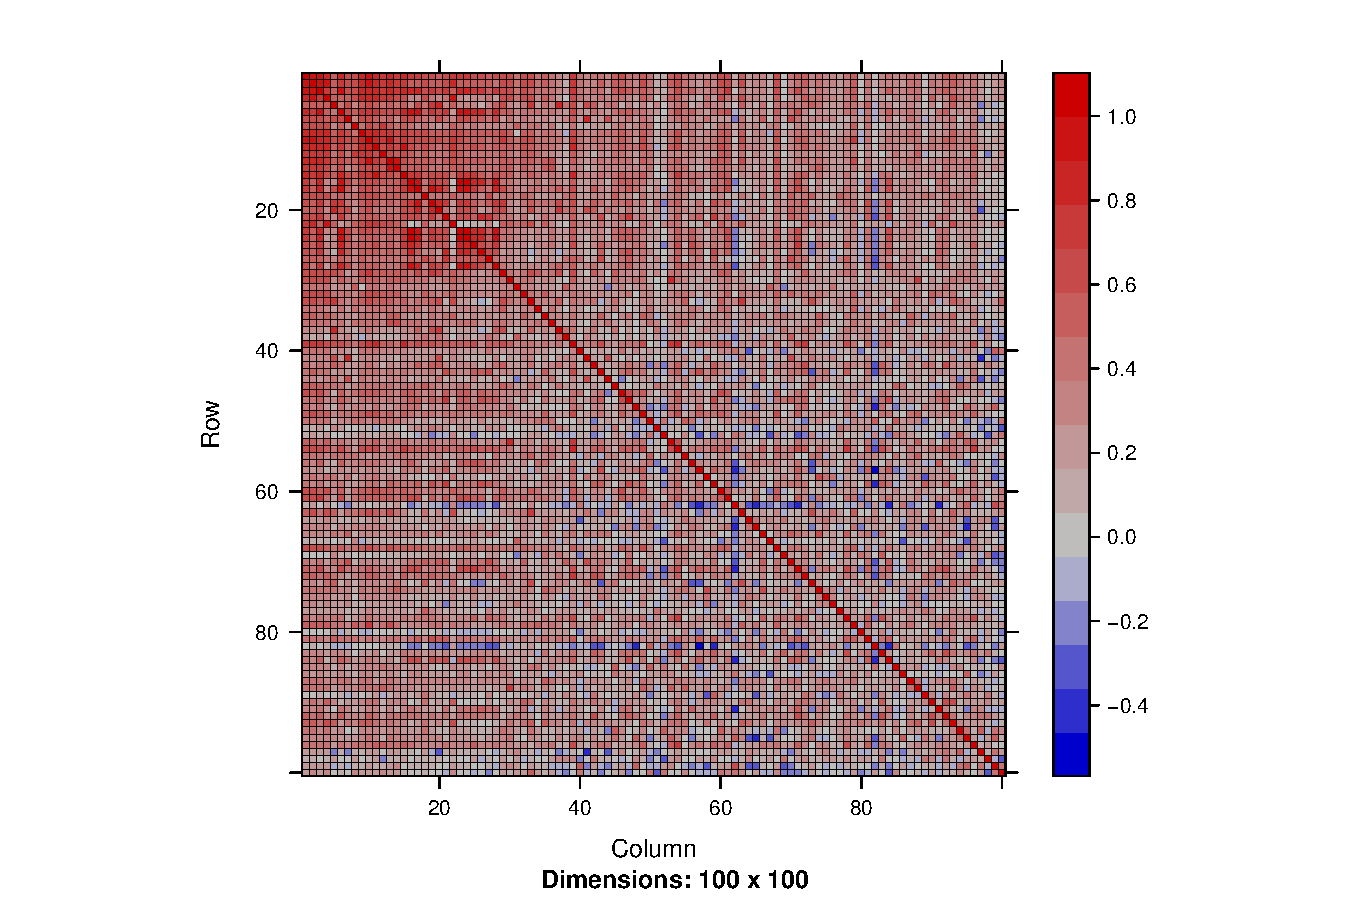
\includegraphics[width=.8\textwidth]{figures/get_plasmodium_data_fig-1} 

\end{knitrout}
\end{frame}

\begin{frame}[containsverbatim,allowframebreaks]
\frametitle{Network between the genes}
\framesubtitle{Sparse Estimation}

Regulatory network between the 100 most variable genes.

\begin{knitrout}\scriptsize
\definecolor{shadecolor}{rgb}{0.969, 0.969, 0.969}\color{fgcolor}\begin{kframe}
\begin{alltt}
\hlkwd{library}\hlstd{(huge)}
\hlstd{huge.out} \hlkwb{<-} \hlkwd{huge}\hlstd{(}\hlkwd{as.matrix}\hlstd{(}\hlkwd{t}\hlstd{(Y[genes.subset, ])),} \hlkwc{method}\hlstd{=}\hlstr{"glasso"}\hlstd{,} \hlkwc{cov.output}\hlstd{=}\hlnum{TRUE}\hlstd{)}
\end{alltt}
\begin{verbatim}
## Conducting the graphical lasso (glasso) with lossless screening....in progress:0% 
Conducting the graphical lasso (glasso) with lossless screening....in progress:9% 
Conducting the graphical lasso (glasso) with lossless screening....in progress:19% 
Conducting the graphical lasso (glasso) with lossless screening....in progress:30% 
Conducting the graphical lasso (glasso) with lossless screening....in progress:40% 
Conducting the graphical lasso (glasso) with lossless screening....in progress:50% 
Conducting the graphical lasso (glasso) with lossless screening....in progress:60% 
Conducting the graphical lasso (glasso) with lossless screening....in progress:70% 
Conducting the graphical lasso (glasso) with lossless screening....in progress:80% 
Conducting the graphical lasso (glasso)....done.                                          
\end{verbatim}
\begin{alltt}
\hlkwd{plot}\hlstd{(huge.out)}
\end{alltt}
\end{kframe}
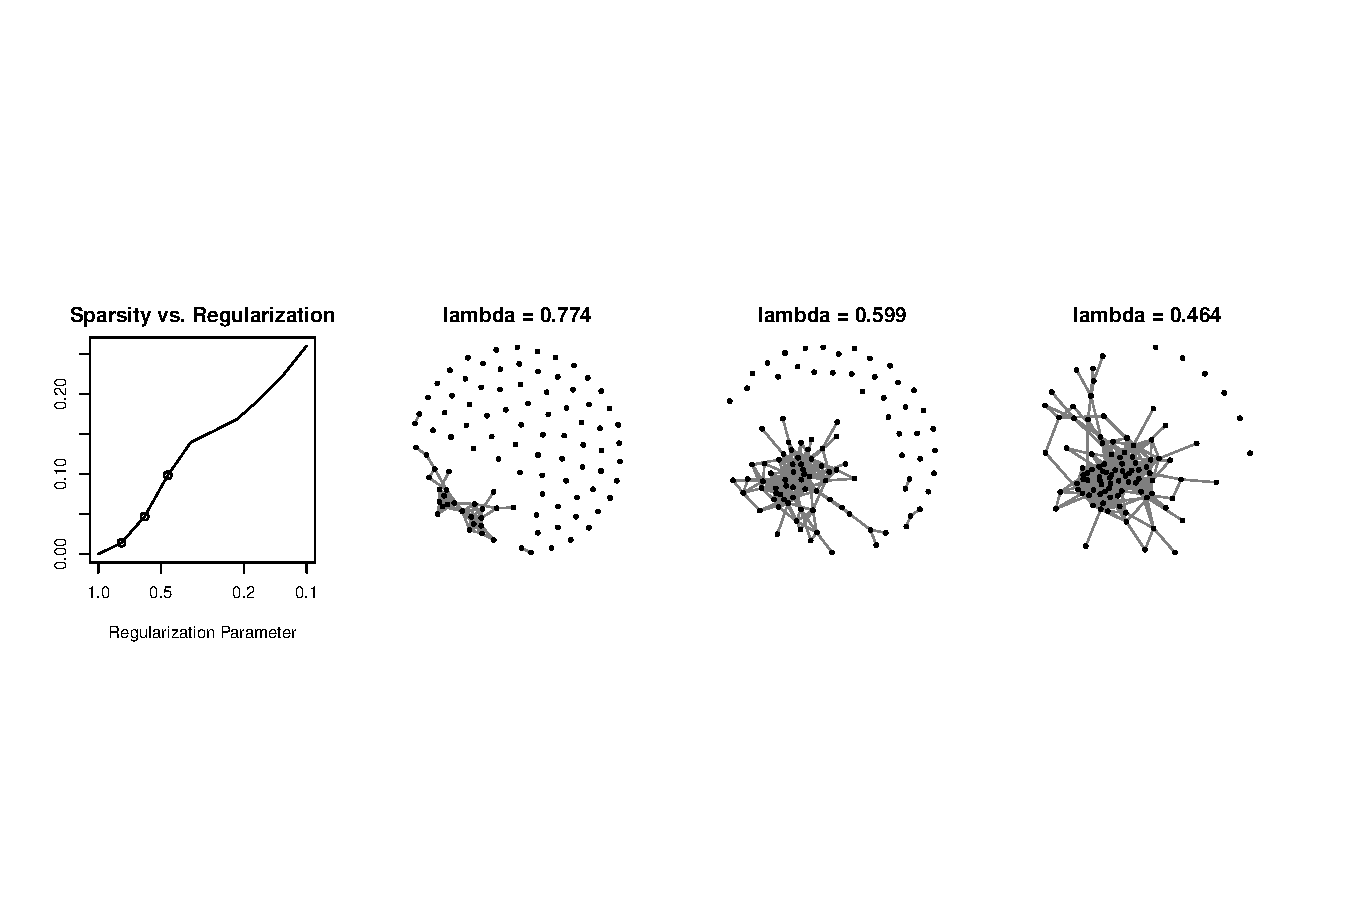
\includegraphics[width=.8\textwidth]{figures/r_show_plasmodium_glasso3-1} 

\end{knitrout}
\end{frame}

\begin{frame}[containsverbatim,allowframebreaks]
\frametitle{Network between the genes}
\framesubtitle{Inverse covariance}

\begin{knitrout}\scriptsize
\definecolor{shadecolor}{rgb}{0.969, 0.969, 0.969}\color{fgcolor}\begin{kframe}
\begin{alltt}
\hlkwd{library}\hlstd{(huge)}
\hlstd{huge.out}\hlopt{$}\hlstd{df}
\end{alltt}
\begin{verbatim}
##  [1]    0   71  233  488  693  763  836  963 1110 1289
\end{verbatim}
\begin{alltt}
\hlkwd{image}\hlstd{(}\hlkwd{Matrix}\hlstd{(huge.out}\hlopt{$}\hlstd{icov[[}\hlnum{3}\hlstd{]]))}
\end{alltt}
\end{kframe}
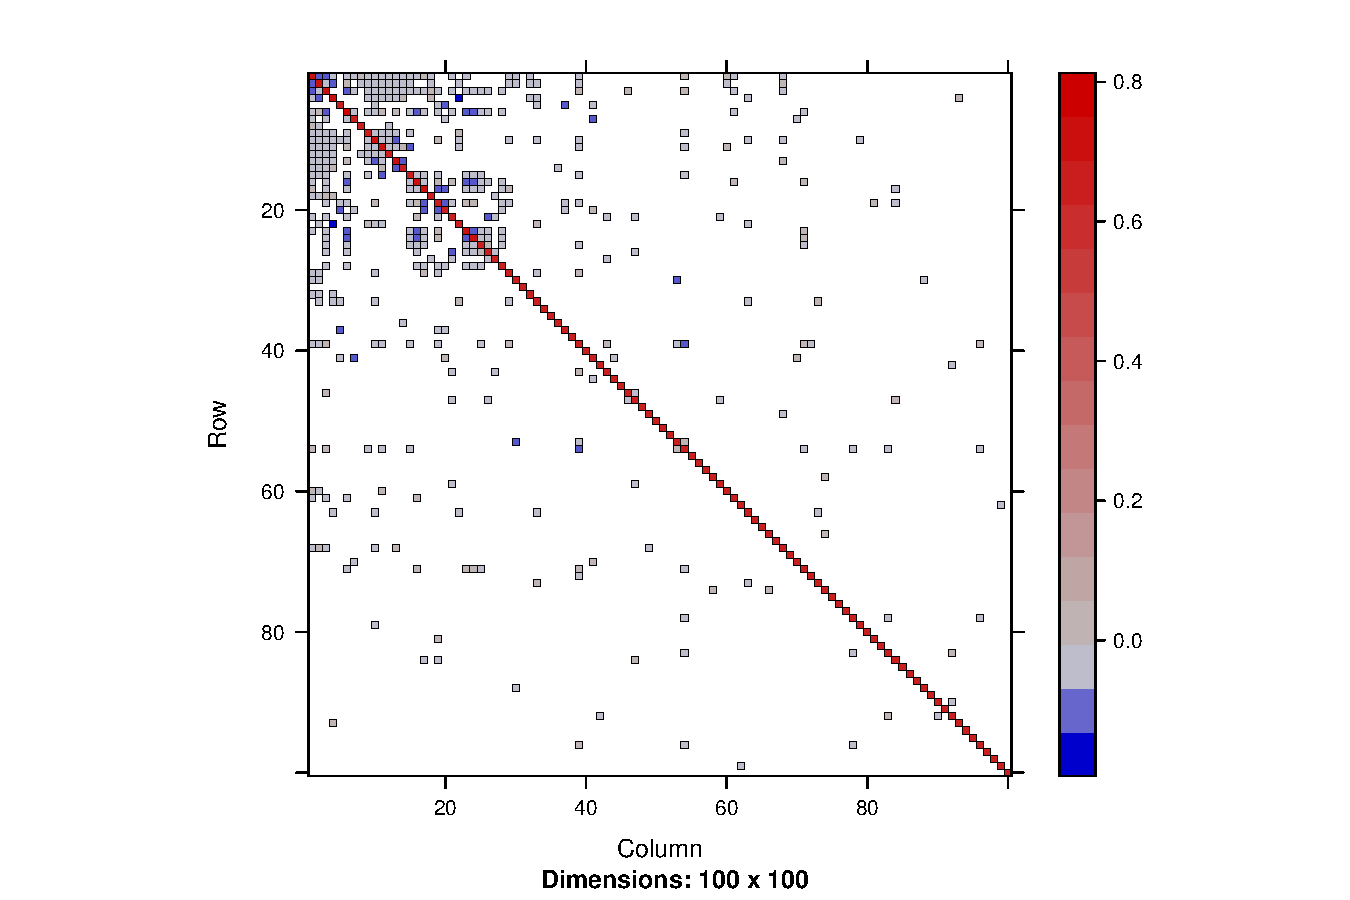
\includegraphics[width=.8\textwidth]{figures/r_show_plasmodium_glasso4-1} 

\end{knitrout}
\end{frame}

\begin{frame}[fragile]
\frametitle{The plasmodium data}
\framesubtitle{Covariance between conditions}

\begin{knitrout}\scriptsize
\definecolor{shadecolor}{rgb}{0.969, 0.969, 0.969}\color{fgcolor}\begin{kframe}
\begin{alltt}
\hlkwd{image}\hlstd{(}\hlkwd{Matrix}\hlstd{(}\hlkwd{cor}\hlstd{(Y)))}
\end{alltt}
\end{kframe}
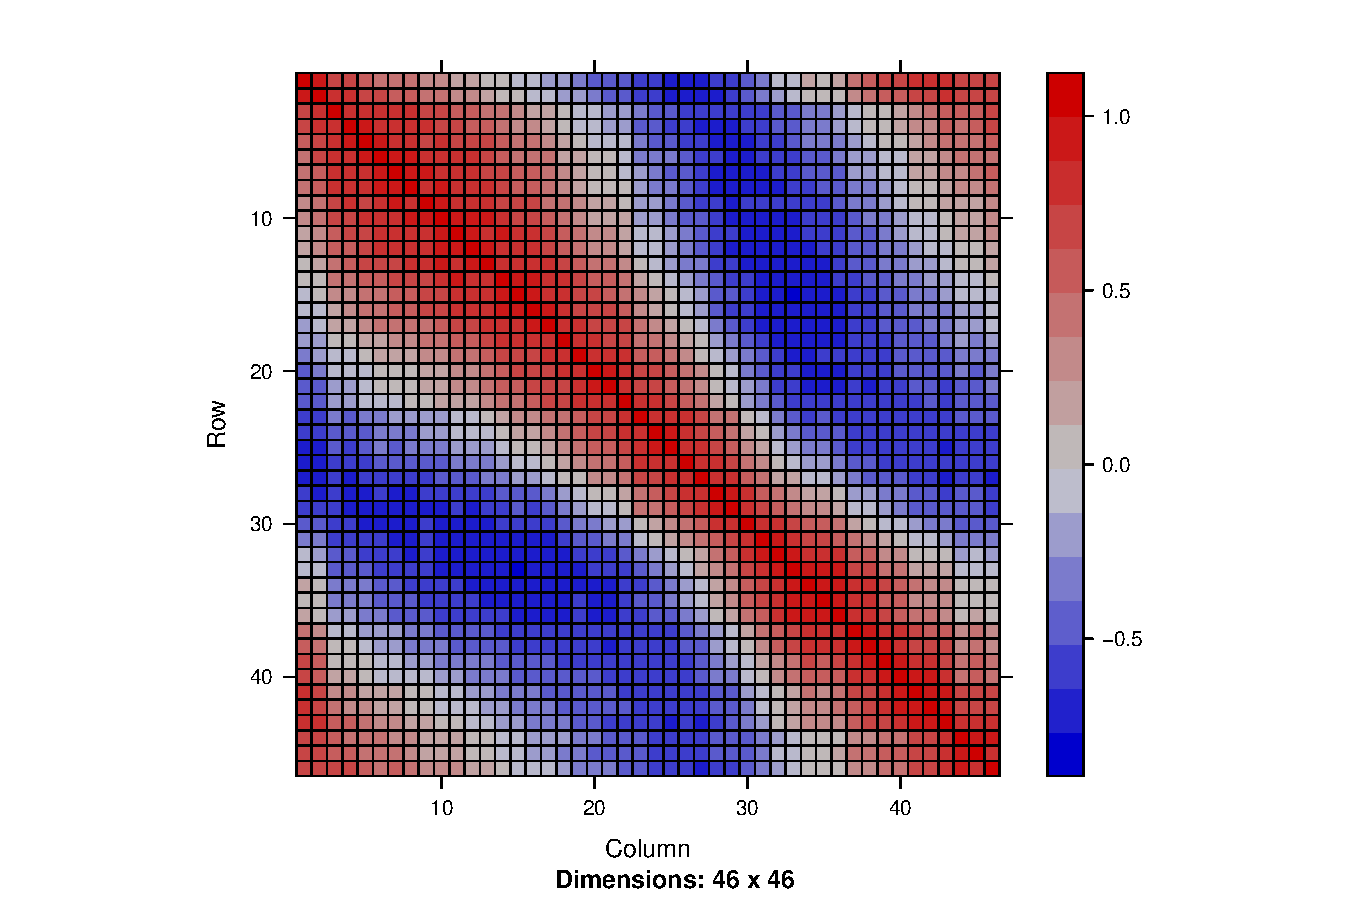
\includegraphics[width=.8\textwidth]{figures/get_plasmodium_data_fig_cond-1} 

\end{knitrout}
\end{frame}

\begin{frame}[containsverbatim]
\frametitle{Covariance structure between the conditions}
\framesubtitle{Sparse Estimation}

\begin{knitrout}\scriptsize
\definecolor{shadecolor}{rgb}{0.969, 0.969, 0.969}\color{fgcolor}\begin{kframe}
\begin{alltt}
\hlkwd{library}\hlstd{(huge)}
\hlstd{huge.out} \hlkwb{<-} \hlkwd{huge}\hlstd{(}\hlkwd{as.matrix}\hlstd{(Y),} \hlkwc{method}\hlstd{=}\hlstr{"glasso"}\hlstd{,} \hlkwc{cov.output}\hlstd{=}\hlnum{TRUE}\hlstd{)}
\end{alltt}
\begin{verbatim}
## Conducting the graphical lasso (glasso) with lossless screening....in progress:0% 
Conducting the graphical lasso (glasso) with lossless screening....in progress:9% 
Conducting the graphical lasso (glasso) with lossless screening....in progress:19% 
Conducting the graphical lasso (glasso) with lossless screening....in progress:30% 
Conducting the graphical lasso (glasso) with lossless screening....in progress:40% 
Conducting the graphical lasso (glasso) with lossless screening....in progress:50% 
Conducting the graphical lasso (glasso) with lossless screening....in progress:60% 
Conducting the graphical lasso (glasso) with lossless screening....in progress:70% 
Conducting the graphical lasso (glasso) with lossless screening....in progress:80% 
Conducting the graphical lasso (glasso)....done.                                          
\end{verbatim}
\begin{alltt}
\hlstd{sel.out}  \hlkwb{<-} \hlkwd{huge.select}\hlstd{(huge.out)}
\end{alltt}
\begin{verbatim}
## Conducting extended Bayesian information criterion (ebic) selection....done
\end{verbatim}
\end{kframe}
\end{knitrout}
\end{frame}

\begin{frame}[containsverbatim]
\frametitle{Covariance structure between the conditions}
\framesubtitle{Sparse Estimation}

\begin{knitrout}\scriptsize
\definecolor{shadecolor}{rgb}{0.969, 0.969, 0.969}\color{fgcolor}\begin{kframe}
\begin{alltt}
\hlkwd{image}\hlstd{(sel.out}\hlopt{$}\hlstd{opt.cov)}
\end{alltt}
\end{kframe}
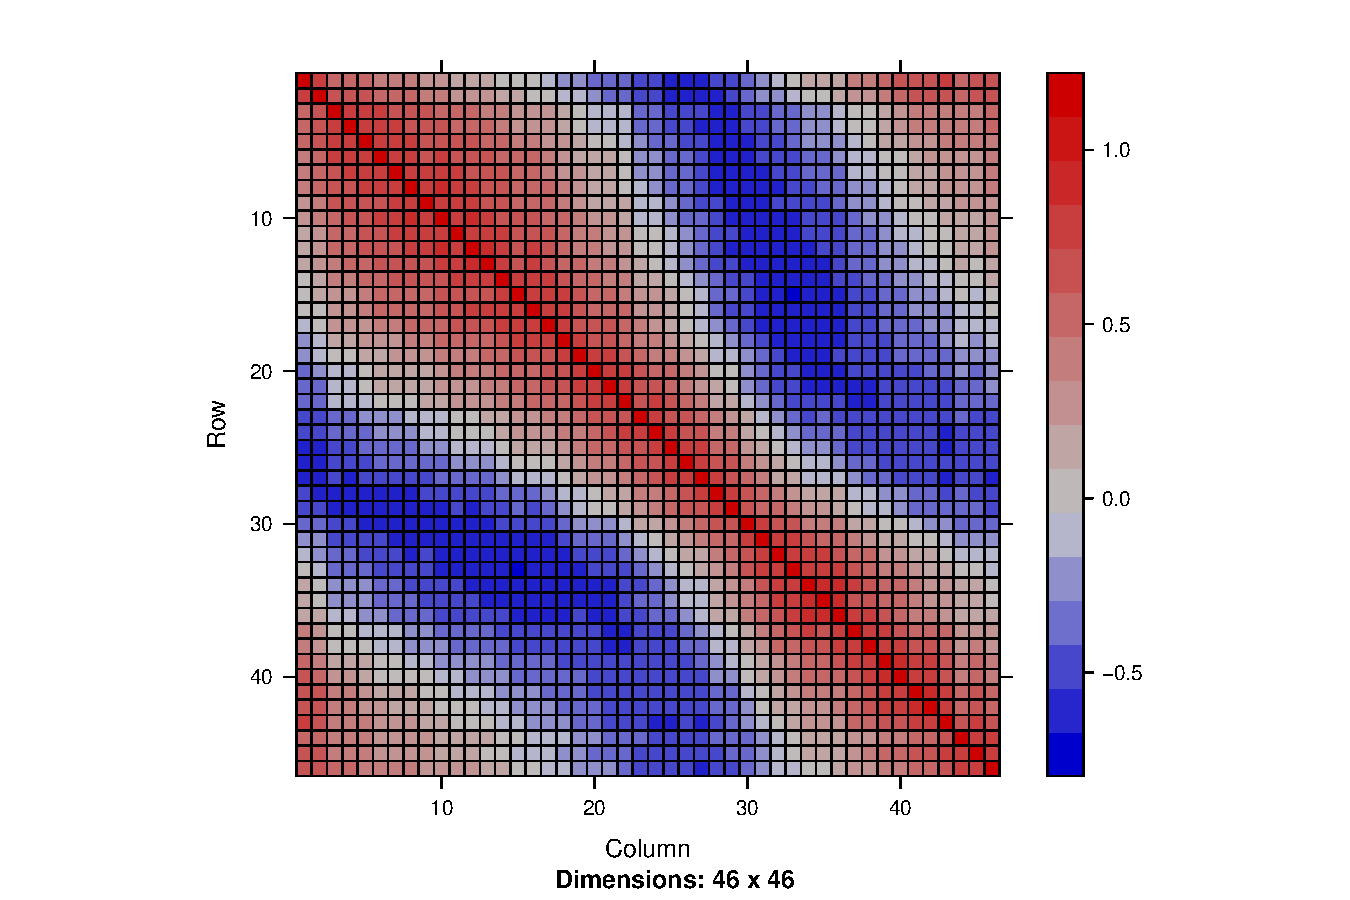
\includegraphics[width=.8\textwidth]{figures/r_get_plasmodium_glassob-1} 

\end{knitrout}
\end{frame}

\begin{frame}[containsverbatim,allowframebreaks]
\frametitle{Covariance structure between the conditions}
\framesubtitle{Sparse Estimation of the inverse covariance}

\begin{knitrout}\scriptsize
\definecolor{shadecolor}{rgb}{0.969, 0.969, 0.969}\color{fgcolor}\begin{kframe}
\begin{alltt}
\hlkwd{sum}\hlstd{(}\hlkwd{abs}\hlstd{(sel.out}\hlopt{$}\hlstd{opt.icov)} \hlopt{!=} \hlnum{0}\hlstd{)}
\end{alltt}
\begin{verbatim}
## [1] 760
\end{verbatim}
\begin{alltt}
\hlkwd{ncol}\hlstd{(sel.out}\hlopt{$}\hlstd{opt.icov)} \hlopt{**} \hlnum{2}
\end{alltt}
\begin{verbatim}
## [1] 2116
\end{verbatim}
\begin{alltt}
\hlkwd{image}\hlstd{(sel.out}\hlopt{$}\hlstd{opt.icov)}
\end{alltt}
\end{kframe}
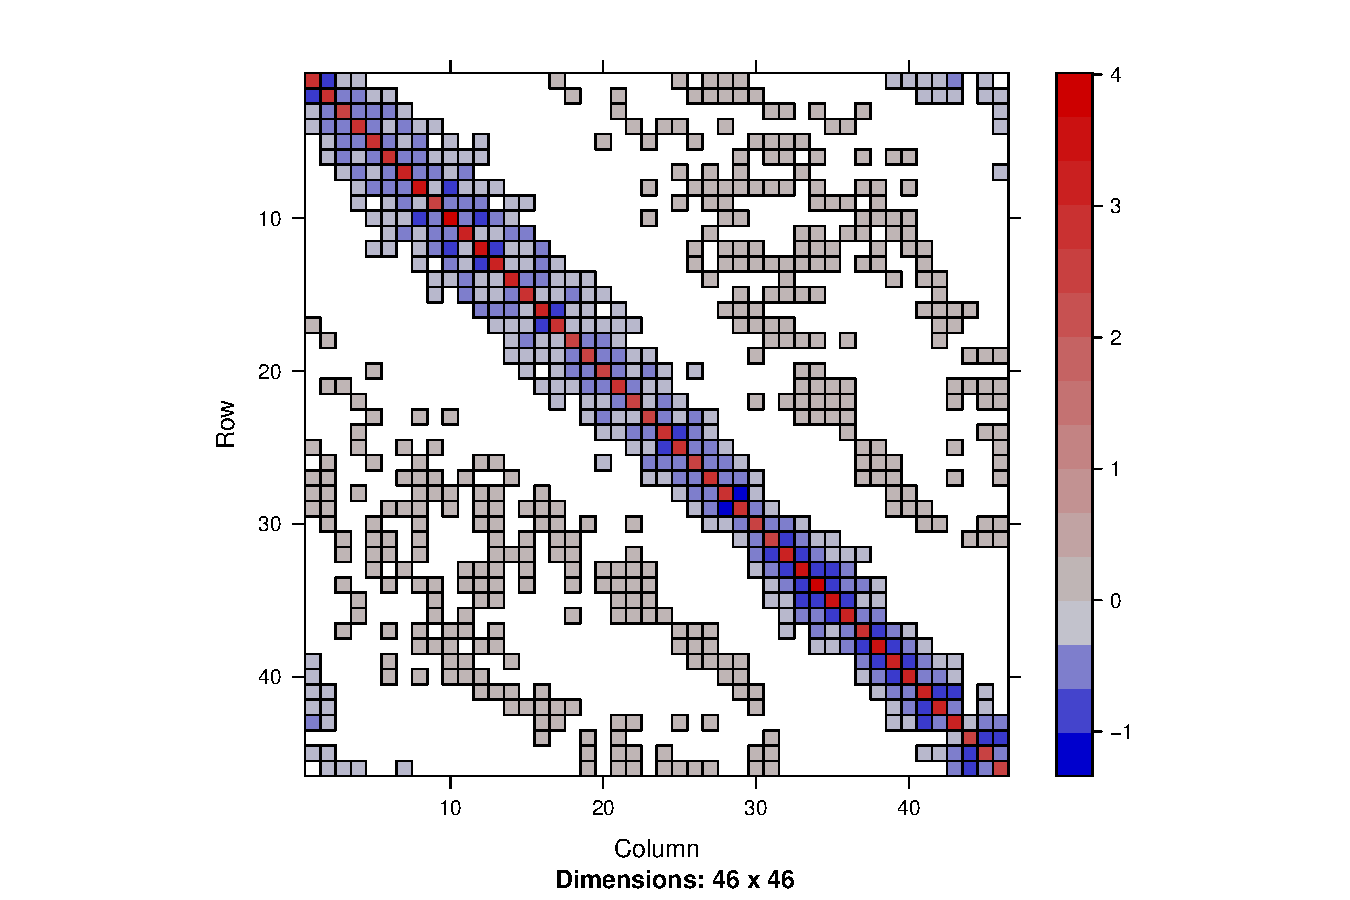
\includegraphics[width=.8\textwidth]{figures/r_show_plasmodium_glasso-1} 

\end{knitrout}

\end{frame}

\begin{frame}[containsverbatim,allowframebreaks]
\frametitle{Covariance structure between the conditions}
\framesubtitle{Associated network}

\begin{knitrout}\scriptsize
\definecolor{shadecolor}{rgb}{0.969, 0.969, 0.969}\color{fgcolor}\begin{kframe}
\begin{alltt}
\hlkwd{plot}\hlstd{(huge.out)}
\end{alltt}
\end{kframe}
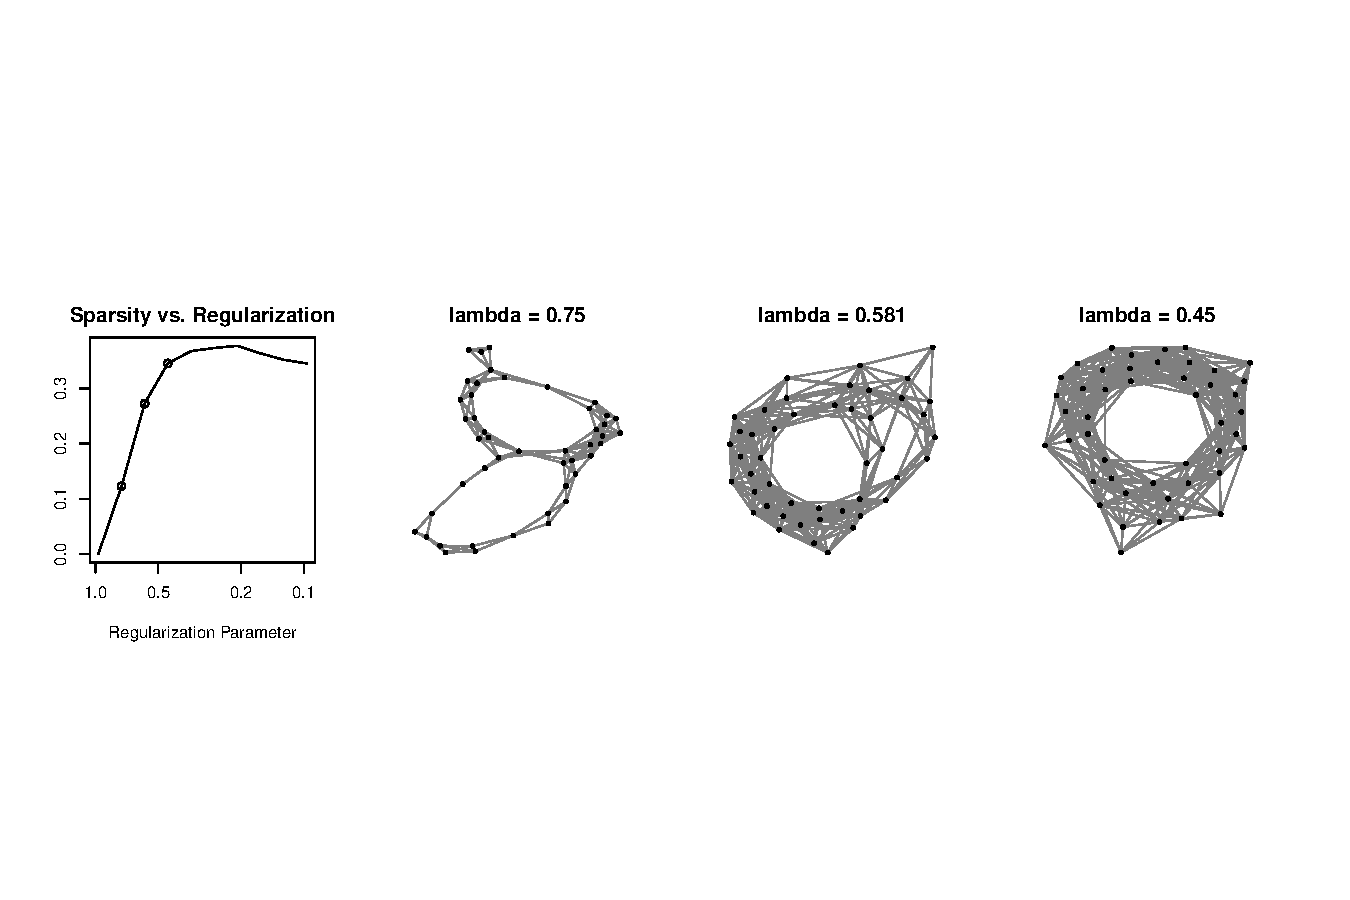
\includegraphics[width=.8\textwidth]{figures/r_show_plasmodium_glasso2-1} 

\end{knitrout}

\end{frame}


